%%%%%%%%%%%%%%%%%%%%%%%%%%%%%%%%%%%%%%%%%%%%%%%%%%%%%%%%%% 
\chapter{クイーン支配問題}\label{chap:background}
%%%%%%%%%%%%%%%%%%%%%%%%%%%%%%%%%%%%%%%%%%%%%%%%%%%%%%%%%% 

\section{支配集合問題}
グラフ$G=(V,E)$の頂点の部分集合$S\subset V$とその隣接頂点の集合との和集合が$V$と一致するとき,$S$を$G$の\textbf{支配集合}という.\par
支配集合$S$の要素数を\textbf{サイズ}という.
 \begin{itemize}
  \item サイズが最小の支配集合を\textbf{最小支配集合}という.
  \item 最小支配集合のサイズをグラフ$G$の\textbf{支配数}と呼ぶ.本論文ではグラフ$G$の支配数を$\gamma(G)$で表す.
 \end{itemize}
  グラフ$G$と正の整数$k$が与えられたとき,サイズが$k$の$G$の支配集合が存在するかどうかを判定する問題を\textbf{支配集合問題}という.
\section{クイーン支配問題}
$n\times n$のチェス盤について各マスを頂点とし,クイーンが移動できるマス同士が辺で結ばれているグラフを\textbf{クイーングラフ}という.サイズ$n\times n$のクイーングラフを$Q_n$で表す.\par
例えば,サイズ3のチェス盤とクイーングラフ$Q_3$の対応関係は図~\ref{ex:queengraph_3}のようになる.
 \begin{figure}[tb]
   \centering
   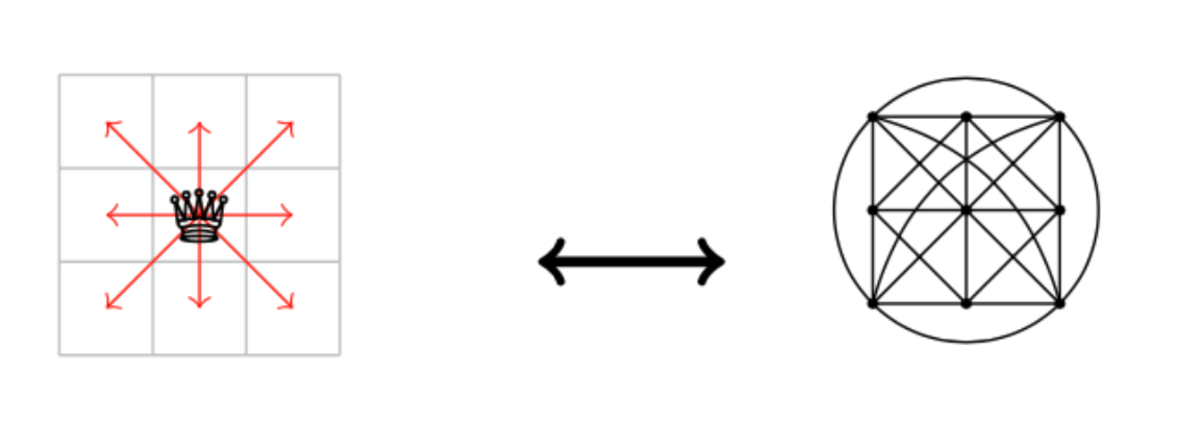
\includegraphics[width=1.0\linewidth]{fig/fig-queen_3_graph.pdf}
   \caption{$3 \times 3$のチェス盤とクイーングラフ$Q_3$の対応関係}
   \label{ex:queengraph_3}
 \end{figure}
クイーングラフ$Q_n$と正の整数$k$が与えられたとき,サイズ$k$の$Q_n$の支配集合が存在するかどうか判定する問題を\textbf{クイーン支配問題}という.\par

クイーングラフ$Q_n$に対する既知の支配数$\gamma(Q_n)$は,表~\ref{tb:queen_n}の通りである.
\begin{table}[hbtp]
   \centering
   \label{tb:queen_n}
   \caption{$n$と$\gamma(Q_n)$の対応表}
   \begin{tabular}{|c|c||c|c||c|c||c|c|} \hline
    $n$ & $\gamma(Q_{n})$ & $n$ & $\gamma(Q_{n})$ &$n$ & $\gamma(Q_{n})$ &$n$ & $\gamma(Q_{n})$ \\ \hline \hline
    1 &1 &6 &3 &11 &5 &16 &9 \\ \hline
    2 &1 &7 &4 &12 &6 &17 &9 \\ \hline
    3 &1 &8 &5 &13 &7 &18 &9 \\ \hline
    4 &2 &9 &5 &14 &8 &19 &10 \\ \hline
    5 &3 &10 &5 &15 &9 &20 &11 \\ \hline
   \end{tabular}
  \end{table}

図\ref{ex:queengraph5}は,$Q_5$の最小支配集合の例である.3個のクイーンを置いたとき,クイーンを移動させて全てのマスにアタック可能である.また,2個以下のクイーンを置いたとき,クイーンを移動させて全てのマスにアタックすることは不可能である.
\begin{figure}[htb]
  \centering
  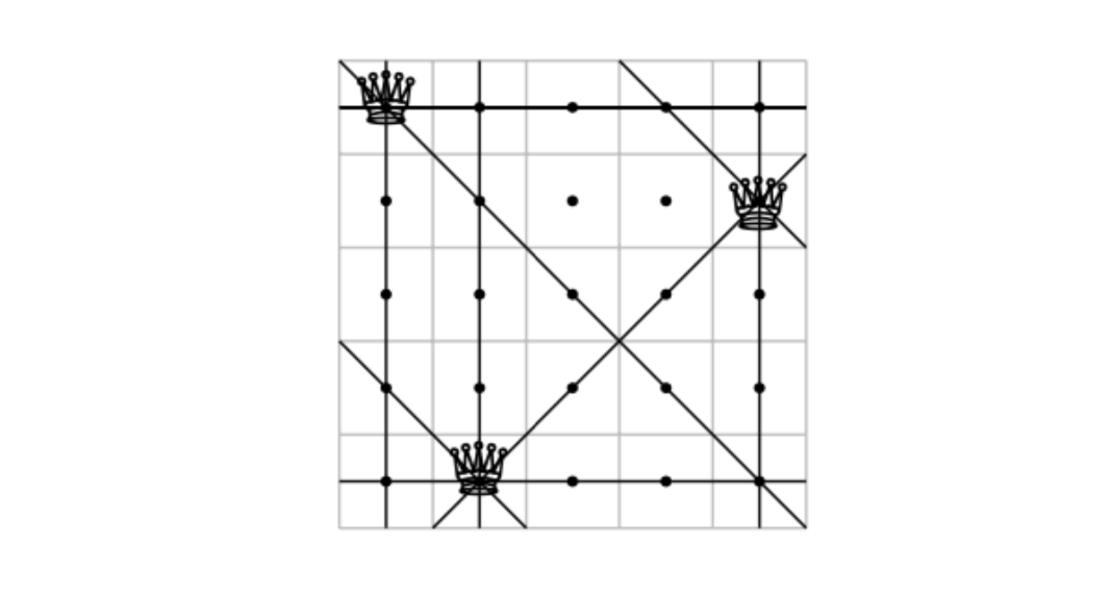
\includegraphics[width=1 \linewidth]{fig/fig-queen_5.pdf}
  \caption{$Q_5$の最小支配集合の例}
  \label{ex:queengraph5}
\end{figure}

%%% Local Variables:
%%% mode: latex
%%% TeX-master: "paper"
%%% End:
